\documentclass[12pt, twocolumn]{article}
\usepackage[utf8]{inputenc}
\usepackage{graphicx}
\graphicspath{ {./figures/} }
\setlength{\columnsep}{0.50cm}

\title{\Huge{\textbf{Assignment1}}}
\author{Prasham Walvekar (CS21BTECH11047)}
\date{March 29, 2022}

\begin{document}

\maketitle

\section*{\large{ICSE 2017 Board Paper Question 4(c):}}
\large{Solve the following inequation and represent the solution set on a number line}
$-8\frac{1}{2} < -\frac{1}{2} - 4x \leq 7\frac{1}{2},$  $x$ \in I.\\
\section*{\large{Solution:}}\\
$-8\frac{1}{2} < -\frac{1}{2} - 4x \leq 7\frac{1}{2}$\\\\
$\Rightarrow -\frac{17}{2} < -\frac{1}{2} - 4x \leq \frac{15}{2}$\\\\
$\Rightarrow -\frac{17}{2} + \frac{1}{2} < -4x \leq \frac{15}{2} + \frac{1}{2}$\\\\
$\Rightarrow-8 < -4x \leq 8$\\\\
Now, dividing the inequality by -4, we get\\
$2 > x \geq -2$\\
(Since on dividing/multiplying an inequality by a negative number, the inequality gets reversed)\\
Hence, we have $-2 \leq x < 2$, and $x$ \in I$\\
Therefore, $x = -2, -1, 0, 1.$ This is the required solution.\\
The solution can be represented on the real number line (as asked in the question): \\
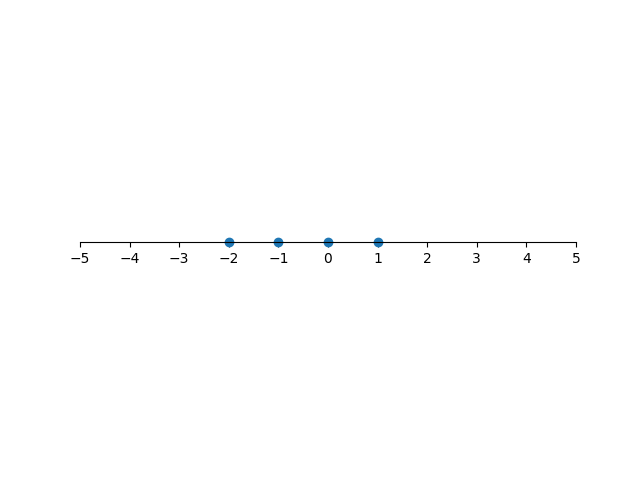
\includegraphics[width=100mm, scale=0.8]{figures/numer_line.png}
The output of the python code used to verify the solution:\\
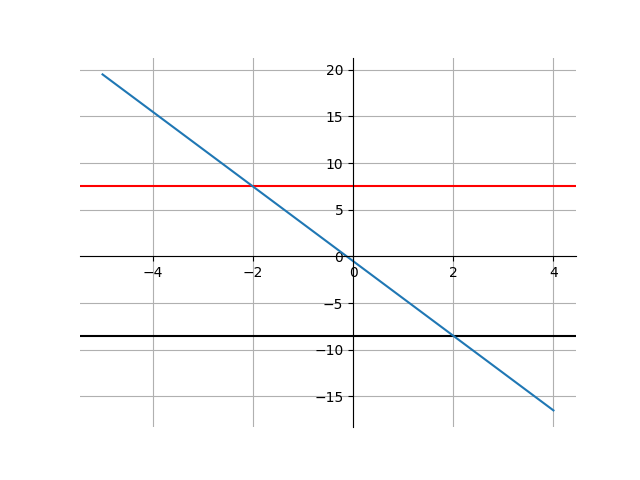
\includegraphics[width=100mm, scale=0.80, left]{figures/line_graph.png}
The graph above contains the lines $y = -\frac{1}{2} - 4x$, $y = -8\frac{1}{2}$, and $y = 7\frac{1}{2}$\\
We need to be concerned about the portion of the line $y = -\frac{1}{2} - 4x$ between the lines $y = -8\frac{1}{2}$, and $y = 7\frac{1}{2}$. The values of x within this portion of line is the required solution, i.e., it can be clearly seen that $y = -\frac{1}{2} - 4x$ intersects $y = -8\frac{1}{2}$ at $x=-2$ and  intersects $y = 7\frac{1}{2}$ at $x=2$. So the range of x would be from -2 to 2 (with $x=2$ excluded).\\
Hence, the answer is verified.


\end{document}

